\section{Entradas Blogue}\label{fich:blogue}

As seguintes seccións amosan o contido das entradas do blogue que se fai en paralelo as clases presenciais. Nesta web publicaranse de forma resumido o explicado nas clases e engadiremos material adicional en forma de vídeos ou artigos da Wikipedia.

\subsection{Elementos básicos: punto, recta e plano}

A xeometría é a rama das matemáticas concernente con cuestións de forma, tamaño, posición relativa de figuras, e coas propiedades do espazo.

Vemos os elementos básicos ou primitivos da xeometría: o punto, a recta e o plano:

Un \textbf{punto} é un elemento ideal/abstracto sen dimensións que serve para representar unha posición do plano. Unha sucesión aliñada de puntos forma unha \textbf{recta}. A recta tamén é un elemento ideal pois so conta con unha dimensión. As rectas son infinitas e non teñen nin principio nin fin. Por último se temos unha conxunto aliñado de rectas e puntos formase un \textbf{plano}.

\begin{center}
    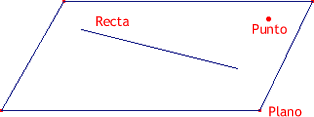
\includegraphics[width=0.5\textwidth]{img/puntorectaplano.png}
\end{center}

As rectas non teñen nin principio nin fin. Se collemos un punto dunha recta, este punto divide a recta en dúas \textbf{semirrectas}. As semirrectas teñen principio pero non teñen fin. Se collemos dous puntos dunha recta o fragmento da recta entre eses dous puntos é un \textbf{segmento}.

Se temos dúas rectas dependendo da súa posición relativa temos diversos tipos:

\begin{center}
    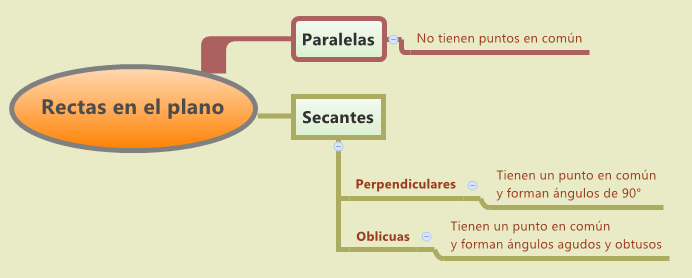
\includegraphics[width=0.9\textwidth]{img/tiposrectas.png}
\end{center}

Vemos algún exemplo do MundoReal sobre rectas paralelas e secantes:

\begin{center}
    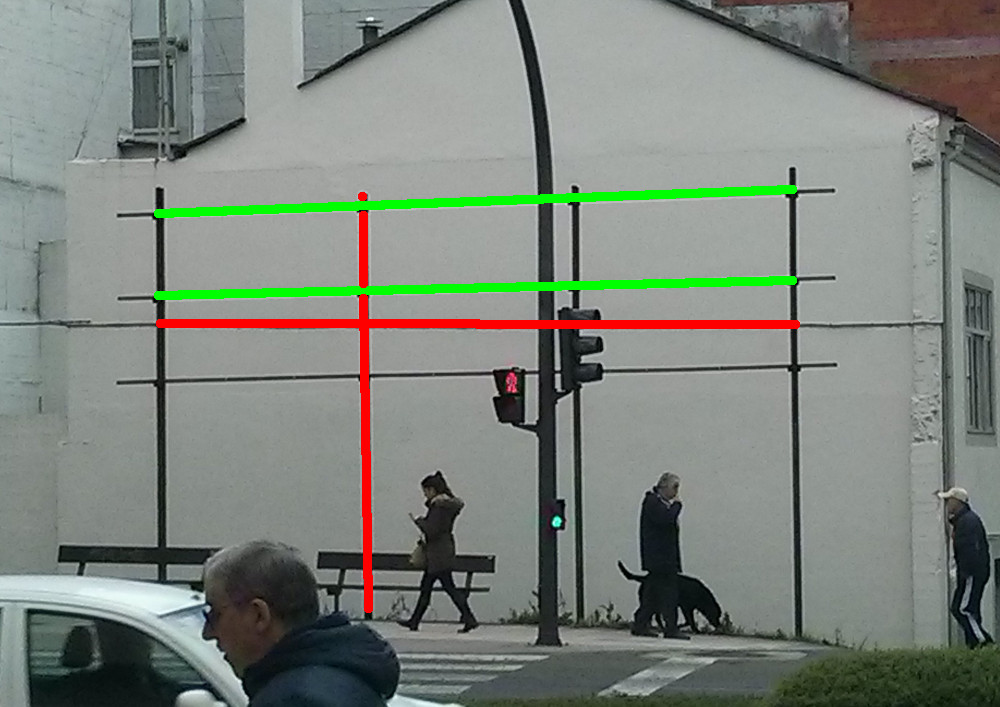
\includegraphics[width=0.8\textwidth]{img/ejemplorectas.jpg}
\end{center}

As rectas verdes son paralelas e as vermellas, secantes.

Como \textbf{recursos adicionais} empregaremos o libro de texto, \cite{yt:puntorecta1} e \cite{yt:semirecta}.


\subsection{Elementos básicos: o ángulo. Sistema Sesaxesimal.}
Un \textbf{ángulo} é a rexión do plano definida por dúas semirrectas que teñen o seu inicio no mesmo punto. A este punto chámaselle \emph{vértice} e as semirrectas, \emph{lados}.

\begin{center}
    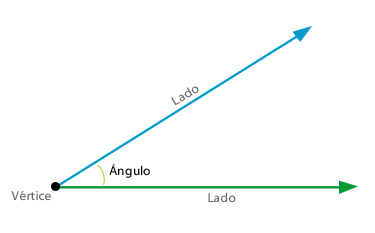
\includegraphics[width=0.5\textwidth]{img/angulo.jpg}
\end{center}

Os ángulos mídense segundo a súa amplitude e unha das unidades de medida son os grados sesaxesimais. Un \textbf{grao} é a $1/360$ parte dun ángulo completo. Cada grado sesaxesimal divídese en \textbf{minutos} e este a súa vez en \textbf{segundos}. Vemos como se calcula a suma e resta de ángulos.

Distinguimos varios tipos ángulos dependendo da súa amplitude:
\begin{itemize}
    \item Completo ($360^{\circ}$)
    \item Cóncavo ($180^{\circ}$)
    \item Llano ($> 180^{\circ}$)
    \item Convexo ($< 180^{\circ}$)
        \begin{itemize}
            \item Obtuso ($> 90^{\circ}$)
            \item Recto ($90^{\circ}$)
            \item Agudo ($< 90^{\circ}$)
            \item Nulo ($0^{\circ}$)
        \end{itemize}
\end{itemize}

Ademais distinguimos varios tipos de ángulos segundo a súa posición relativa:

\begin{itemize}
    \item Ángulos consecutivos: comparten un lado.
    \item Ángulos adxacentes: ángulos consecutivos que teñen o lado común sobre a mesma recta.
    \item Ángulos opostos polo vértice.
\end{itemize}

Facemos exercicios nos que se pide indicar o tipo de ángulo. Sacamos os ángulos de \href{https://www.random.org}{www.random.org}.

Como \textbf{recursos adicionais} empregaremos o libro de texto, \cite{wiki:angulos}, \cite{yt:angulostriangulos}, \cite{yt:sumarestasexagesimal} e \cite{yt:sumaresta}.

\subsection{Mediatriz e bisectriz}

A mediatriz dun segmento é a recta cuxos puntos equidistan dos dous extremos do segmento. Graficamente calcúlase cun compás, determinándose coa intersección de dous arcos que teñan o seu centro nos extremos do segmento e o mesmo raio (superior á metade do segmento, se non non chegan a cortarse).

\begin{center}
    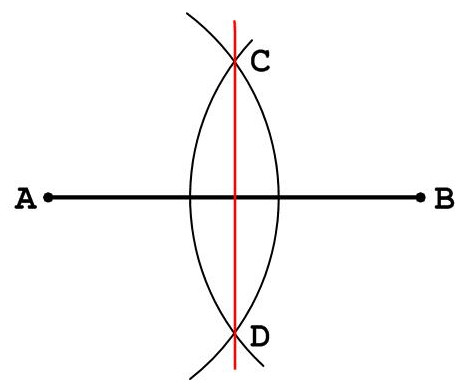
\includegraphics[width=0.3\textwidth]{img/mediatriz.jpg}
\end{center}

A bisectriz dun ángulo é a recta cuxos puntos equidistan dos lados do ángulo. Graficamente calcúlase cun compás, determinándose a mediatriz entre dous puntos M e N das rectas que estean á mesma distancia do vértice A.

\begin{center}
    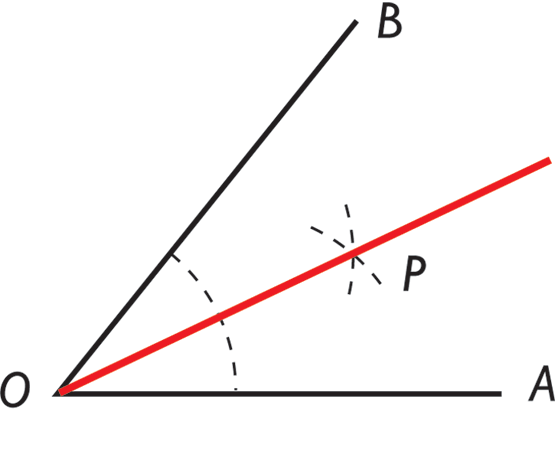
\includegraphics[width=0.3\textwidth]{img/bisectriz.png}
\end{center}

Como \textbf{recursos adicionais} empregaremos o libro de texto e \cite{yt:bisectrizmediatriz}.

\subsection{Liña Poligonal. Polígonos. Triángulos}

Unha liña poligonal é a que se forma cando unimos segmentos de recta dun plano. Es esta liña é cerrada, é dicir, se o extremo do primeiro segmento coincide co do último; definen unha rexión do plano que denominamos polígono.

\begin{center}
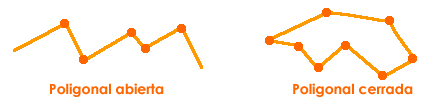
\includegraphics[width=0.75\textwidth]{img/lineapoligonal.jpg}
\end{center}

Os segmentos que definen un polígono denomínanse lados e os extremos destes segmentos, vértices. Se unimos dous vértices non consecutivos obtemos as diagonais.

Un polígono pode ser cóncavo se ten algún ángulo cóncavo ou convexo se todos os seus ángulos son convexos. Ademais se todos os seus ángulos e lados son iguais entre si, denomínase regular e no caso contrario, irregular.

O triángulo é o polígono de 3 lados. Clasificamos os triángulos en función de dous parámetros:

\begin{itemize}
    \item Ángulos do triángulo
    \begin{itemize}
        \item Acutángulo $\,\to\,$ Todos os ángulos agudos ($< 90^{\circ}$).
        \item Rectángulo $\,\to\,$ Teñen un ángulo recto ($90^{\circ}$).
        \item Obtusángulo $\,\to\,$ Teñen un ángulo obtuso ($> 90^{\circ}$).
    \end{itemize}
    \item Número de lados que teñen iguais.
    \begin{itemize}
        \item Equilátero $\,\to\,$ Todos os seus lados iguais.
        \item Isósceles $\,\to\,$ Teñen 2 lados iguais.
        \item Escaleno $\,\to\,$ Todos os seus lados distintos.
    \end{itemize}
\end{itemize}

\begin{center}
    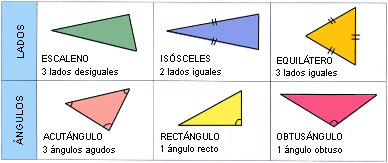
\includegraphics[width=0.9\textwidth]{img/clasiftriangulos.jpg}
\end{center}

Os ángulos dun triángulo sempre suman $180^{\circ}$.

\begin{center}
    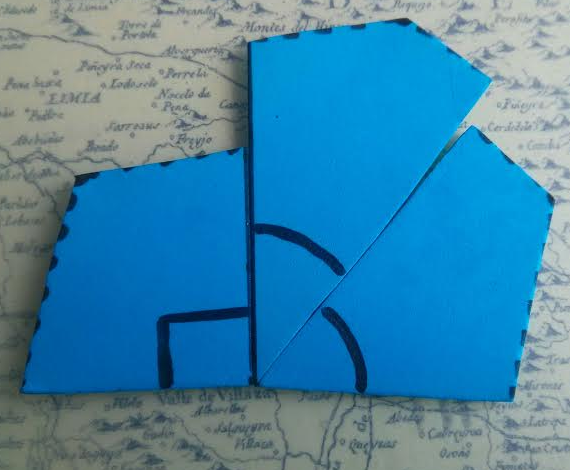
\includegraphics[width=0.35\textwidth]{img/180grados-1.png}
    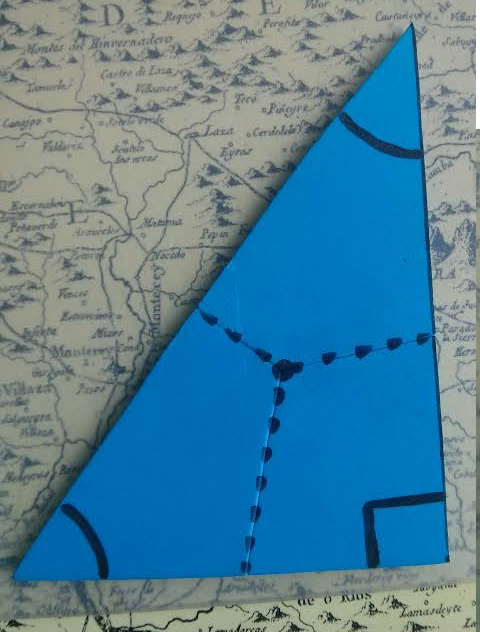
\includegraphics[width=0.35\textwidth]{img/180grados-2.png}
\end{center}

Como \textbf{recursos adicionais} empregaremos o libro de texto e \cite{yt:angulostriangulos}.



\subsection{Puntos e rectas notables do triángulo}

O primeiro punto notable á o circuncentro. O circuncentro é o punto do triángulo tal que equidista dos tres vértices e, polo tanto é centro da circunferencia circunscrita do triángulo. Pódese empregar para por exemplo saber onde localizar unha antena que equidiste dos 3 puntos que se poden ver no plano:

\begin{center}
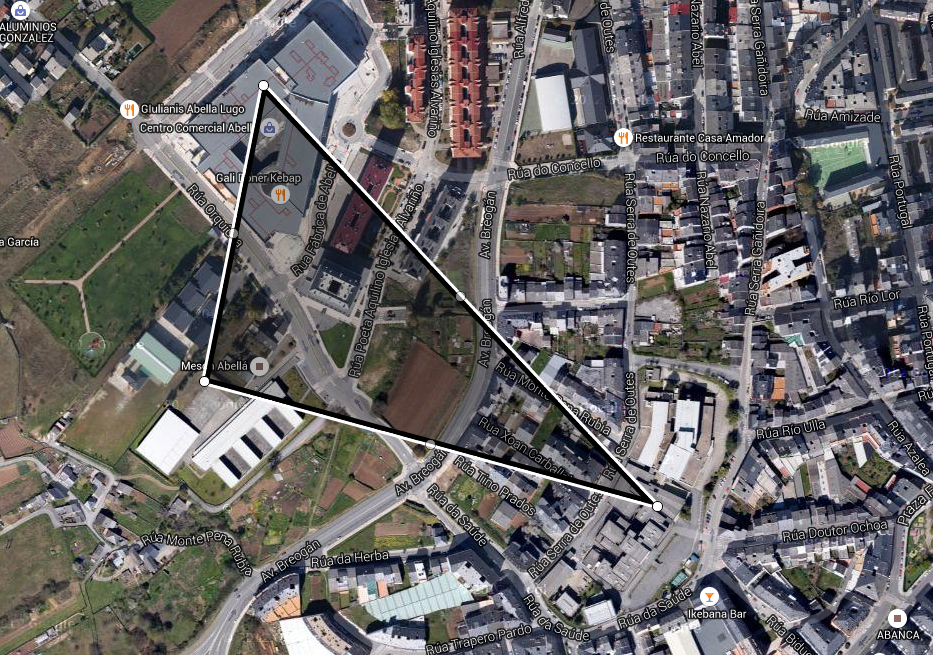
\includegraphics[width=0.6\textwidth]{img/circuncentro.png}
\end{center}

Para trazalo teremos que calcular as mediatrices dos lados. Recordamos que as mediatrices eran as rectas cuxos puntos equidistaban dos dous extremos dun segmento. O punto de corte entre as tres mediatrices do triángulo daranos o punto que equidiste dos 3 vértices (o circuncentro).

Outro punto notable é o incentro que é o centro da circunferencia inscrita (interior) do triángulo.

\begin{center}
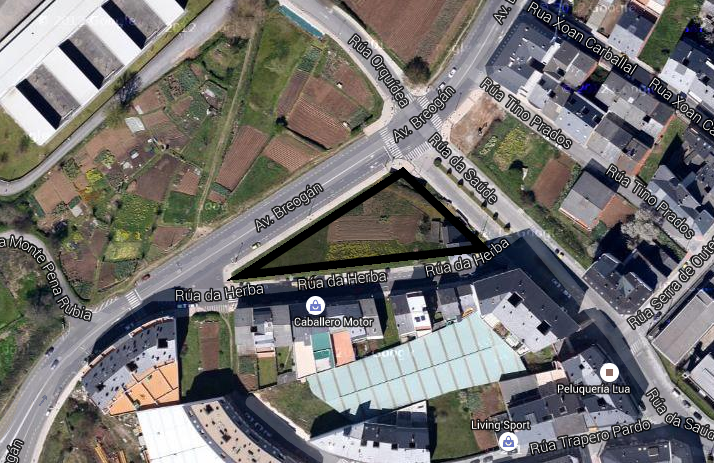
\includegraphics[width=0.6\textwidth]{img/incentro.png}
\end{center}

Para trazala debemos empregar as bisectrices. Lembramos que as bisectrices eran as rectas cuxos puntos equidistaban dos dous lados dun ángulo. Se trazamos as bisectrices dos ángulos dun triángulo, o punto onde se cortan equidista de todos os lados e polo tanto é centro da circunferencia inscrita.

O baricentro representa o centro de gravidade do triángulo e calcúlase trazando as medianas. As medianas son unhas rectas que van dende o punto medio dun lado ao vértice oposto.

\begin{center}
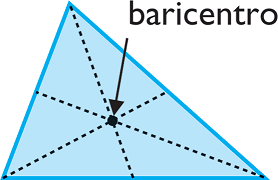
\includegraphics[width=0.3\textwidth]{img/baricentro.png}
\end{center}

Por último as alturas son as rectas perpendiculares a cada lado pasando polo vértice oposto. O punto onde se cortan as alturas denomínase ortocentro.

\begin{center}
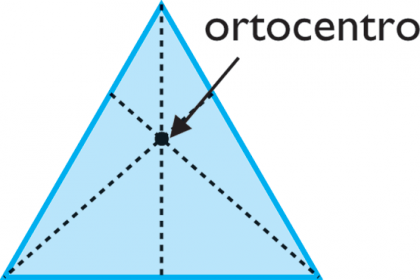
\includegraphics[width=0.3\textwidth]{img/ortocentro.png}
\end{center}

Como \textbf{recursos adicionais} empregaremos o libro de texto, \cite{yt:circuncentro}, \cite{yt:incentro}, \cite{yt:baricentro} e \cite{yt:ortocentro}.

\subsection{Teorema de Pitágoras}

Nun triángulo rectángulo os lados do ángulo recto chámanse catetos e o lado oposto hipotenusa. Tendo en conta isto, o Teorema de Pitágoras establece que a lonxitude ao cadrado da hipotenusa é igual a suma das lonxitudes dos catetos ao cadrado:

\begin{center}
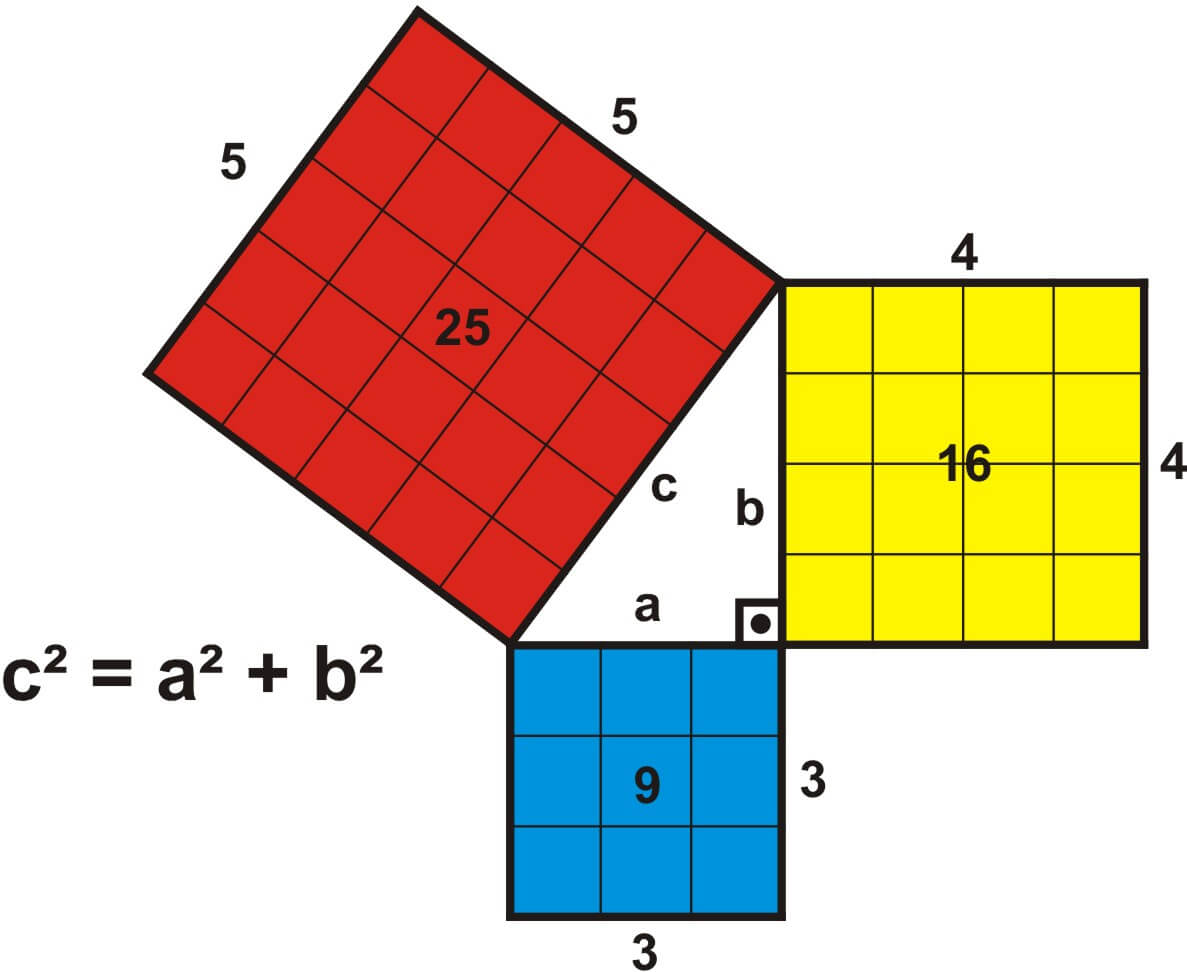
\includegraphics[width=0.6\textwidth]{img/pitagoras1.jpg}
\end{center}

Vemos as demostracións de \cite{yt:pitagoras} e \cite{universomat}.


\subsection{Cuadriláteros}

Os cuadriláteros son os polígonos de 4 lados. A súa clasificación é a seguinte:

\begin{itemize}
    \item Paralelogramos (lados opostos paralelos).
    \begin{itemize}
        \item Cadrado $\,\to\,$ Lados iguais, ángulos iguais
        \item Rectángulo $\,\to\,$ Lados desiguais, ángulos iguais.
        \item Rombo $\,\to\,$ Lados iguais, ángulos desiguais.
        \item Romboide $\,\to\,$ Lados desiguais, ángulos desiguais.
    \end{itemize}
    \item Non paralelogramos
    \begin{itemize}
        \item Trapecio (2 lados paralelos)
        \begin{itemize}
            \item Trapecio isósceles (2 lados iguais)
            \item Trapecio rectángulo (teñen 2 ángulos rectos)
            \item Trapecio Escaleno (Lados desiguais)
        \end{itemize}
    \end{itemize}
    \item Trapezoide (ningún lado paralelo)
\end{itemize}

\begin{center}
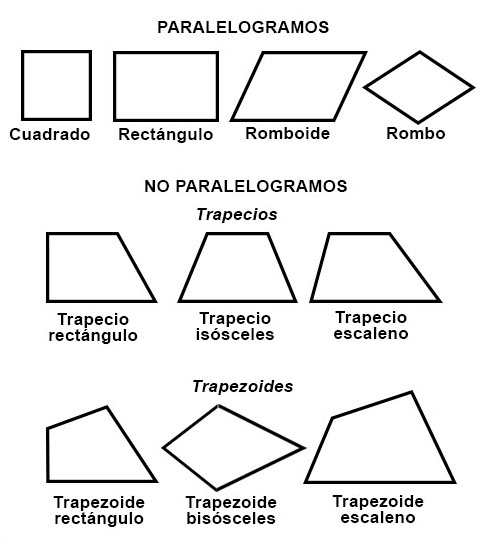
\includegraphics[width=0.8\textwidth]{img/clasificacin-cuadrilateros.jpg}
\end{center}

Como \textbf{recursos adicionais} empregaremos o libro de texto, \cite{wiki:cuadrilatero}, \cite{yt:cuad1} e \cite{yt:cuad2}.
